\chapter{Introducción}
\label{chap:introducción}

\section{Introducción}
¿Qué determina el color de los ojos, la estatura o incluso la predisposición a ciertas condiciones de salud? La respuesta reside en un manual de instrucciones que se encuentra en cada una de nuestras células: nuestro ADN\footnote{Ácido Desoxirribonucleico}. El ADN está compuesto por aproximadamente 3.000 millones de ''letras'' químicas, una secuencia tan extensa que, si se imprimiera, formaría una torre de papel de más de 100 metros de altura\cite{lander2001}. El campo que se dedica a descifrar y a entender cómo se transmiten sus instrucciones entre generaciones es la genética.

Dentro de este inmenso texto genético, los genes actúan como los capítulos; estos son fragmentos específicos de ADN que contienen la información necesaria para manifestar un rasgo biológico, desde la apariencia física hasta el comportamiento. Estos genes se organizan en estructuras mayores llamadas cromosomas, que no solo los contienen, sino que también interactúan con el entorno y se ven influenciados por nuestro estilo de vida para orquestar el complejo funcionamiento del organismo\cite{robinson}. 

A pesar de que los seres humanos compartimos más del 99\% del ADN, es en ese pequeño porcentaje, el cual está compuesto por lo que se llaman variantes genéticas, donde reside la variabilidad individual. Las variantes genéticas son diferencias en la secuencia del ADN que distinguen a los individuos entre sí y son responsables del color de ojos o la estatura (características fenotípicas). Sin embargo, además de su efecto en la apariencia, algunas de estas variantes pueden alterar el funcionamiento de ciertos genes, modificando la probabilidad de desarrollar determinadas enfermedades. Por tanto, la identificación y el estudio de estas variaciones permiten comprender mejor la base genética de muchas patologías e identificar riesgos hereditarios a determinadas enfermedades.  

Las patologías o enfermedades con base genética se pueden diferenciar en simples y complejas, en función del número de genes afectados. Por un lado, las enfermedades simples son más sencillas de diagnosticar y tratar dado que dependen de la alteración en un único gen, la cual tiene un efecto directo y a menudo predecible. Por otro lado, las enfermedades complejas, que constituyen la mayoría de las afecciones comunes, presentan una complejidad mucho mayor por la combinación de múltiples variaciones\cite{visscher}. Esto dificulta el estudio de su patrón genético. Un ejemplo de esta complejidad se observa en las distrofias de retina, donde variaciones en más de 250 genes distintos pueden dar lugar a una patología similar, con un patrón genético que varía significativamente de un paciente a otro.  

Adicionalmente, el desarrollo de las enfermedades complejas no depende únicamente del factor genético, sino que también está fuertemente influenciado por el estilo de vida y los factores medioambientales. Como resultado, el componente genético por sí solo no es un factor determinante, sino que el efecto agregado de numerosas variaciones genéticas aumenta la predisposición a padecer la enfermedad \cite{ye}. 

Su diagnóstico y prevención son de gran relevancia, ya que no solo mejora la calidad de vida de los pacientes, sino que también representa un enfoque más sostenible y costo-efectivo, ayudando a reducir la considerable sobrecarga económica y de recursos que soportan los sistemas de salud.  

Para abordar esta complejidad, la investigación genómica ha desarrollado herramientas estadísticas que permiten agrupar y cuantificar el efecto de estas variantes, como los modelos de Puntuación de Riesgo Poligénico (PRS, del inglés \textit{Polygenic Risk Score})\cite{lewis}. Estos modelos estadísticos son capaces de agregar la información de todas estas pequeñas variantes para calcular una estimación del riesgo genético global de un individuo para una enfermedad específica, convirtiéndose en una herramienta prometedora para la medicina preventiva y personalizada.


\section{Motivación}

Como se ha mencionado anteriormente, en  el campo de la medicina se está observando que los análisis de PRS tienen potencial para mejorar la predicción del riesgo a padecer una enfermedad, incluso cuando ya se consideran factores tradicionales como el historial familiar o riesgos derivados del estilo de vida. Además, estos permiten la predicción de múltiples enfermedades en una sola prueba, por lo que se busca la introducción de estos análisis para complementar los ya existentes. 

A pesar de su gran potencial clínico, la integración de las Puntuaciones de Riesgo Poligénico (PRS) en la práctica clínica enfrenta importantes desafíos, ya que la transición de una herramienta de investigación a una aplicación clínica estándar requiere de \textit{software} que no solo sea preciso, sino también accesible y eficiente para el personal sanitario.

Los artefactos existentes presentan un grado de dificultad elevado comparado con el conocimiento medio que pueda tener una persona no experta en el dominio de la investigación. Por ejemplo, la mayoría de estas herramientas requieren el uso de la línea de comandos (\textit{CLI}) y la configuración manual de ficheros de texto. Esto supone una barrera significativa para la implementación de esta tecnología en un contexto clínico, ya que limita su adopción por parte de profesionales que no disponen de formación técnica avanzada. 

Por ello, en este trabajo se plantea el desarrollo de un \textit{software} que permita a los usuarios no expertos utilizar estas potentes herramientas bioinformáticas. Este objetivo se alcanza reduciendo la carga tecnológica para los usuarios no expertos que potencialmente puedan beneficiarse de esta herramienta. Teniendo una interfaz más amigable para el usuario y con un grado de información más centralizado, permitirá a estos usuarios ejecutar los pasos necesarios para completar un análisis PRS de forma intuitiva.

Formar parte de este proyecto ha supuesto una valiosa oportunidad para colaborar en una línea de trabajo consolidada y desarrollada. Esta iniciativa ha permitido aplicar los conocimientos adquiridos durante el grado para abordar los retos reales a los que se enfrentan los investigadores en el campo de la genética y la medicina. La aportación de este Trabajo de Fin de Grado se enmarca dentro de un objetivo más general y de alto valor añadido: desarrollar herramientas sencillas y accesibles que tengan el potencial de marcar una diferencia significativa en la vida de los pacientes.

\section{Objetivos}

El objetivo general de este trabajo de fin de grado es \textbf{facilitar la ejecución de análisis PRS en contextos clínicos}. Para alcanzar este objetivo, se llevará a cabo el desarrollo de una plataforma web accesible que facilite el análisis PRS para su posterior aplicación. Para la consecución de este objetivo general, se han definido tres objetivos específicos (OE).
\begin{description}
    \item[OE1] Estudiar el contexto: Identificar los fundamentos genéticos, estadísticos y clínicos que sustentan el uso de análisis PRS en la predicción del riesgo de enfermedades complejas. También se analizarán las principales herramientas existentes para llevar a cabo análisis PRS para identificar las limitaciones que presentan. De esa forma, el conocimiento adquirido y las posibilidades de mejora sirven para llevar a cabo un desarrollo más alineado con las necesidades que existen hacia la plataforma.
    \item[OE2] Crear una plataforma web: Desarrollar una plataforma sencilla y accesible que permita el análisis de PRS, incluso para quienes no tienen experiencia en bioinformática. Posteriormente, se estudiarán las herramientas ya existentes y se determinará la complejidad de las herramientas actuales y la necesidad de diseñar una solución que no requiera conocimientos técnicos avanzados y sea sencilla e intuitiva.
    \item[OE3] Validar el sistema: Realizar pruebas para validar y comprobar que el sistema funciona como se espera: se recogerán opiniones de profesionales para entender si la herramienta se adapta a sus necesidades.
\end{description}

\section{Metodología}
\label{section:metodologia}
La metodología de trabajo empleada en este proyecto es la Ciencia del Diseño (\textit{Design Science}). Este enfoque se basa en el marco metodológico definido por Roel J. Wieringa\cite{wieringa}, al cual se hará referencia a lo largo de este apartado.

La metodología \textit{design science} tiene como objetivo principal la búsqueda de soluciones a problemas del mundo real. Más concretamente, se centra en el diseño e investigación de artefactos en un contexto.

En este trabajo, el \textbf{artefacto} es una plataforma web interactiva que facilita los análisis de \textit{Polygenic Risk Scores} y el \textbf{contexto} es el estudio genético de las enfermedades complejas.

El marco de trabajo de Wieringa distingue dos niveles de actuación en la \textit{design science methodology}: el ciclo de ingeniería y el ciclo de diseño. El ciclo de diseño es un subproceso del ciclo de ingeniería, siendo este último el proceso completo que va desde el estudio de un problema hasta la implantación y evaluación de su solución en el mundo real.

Sin embargo, los proyectos de investigación académica como este TFG se centran en las primeras tres fases del ciclo de ingeniería, las cuales constituyen el ciclo de diseño. La razón de este enfoque es que el objetivo principal no es construir una solución con un grado de robustez y escalabilidad de nivel comercial, sino diseñar y validar un artefacto novedoso como prueba de concepto.

Por lo tanto, este ciclo se enfoca en el diseño riguroso del artefacto y, fundamentalmente, en la justificación argumentada de que dicho artefacto, si llegara a implementarse en un entorno real, contribuiría a los objetivos de los interesados. El presente trabajo ejecutará un ciclo de diseño completo, tal y como se ilustra en la Figura~\ref{fig:ciclo_diseno}

\begin{figure}[H]
\centering
    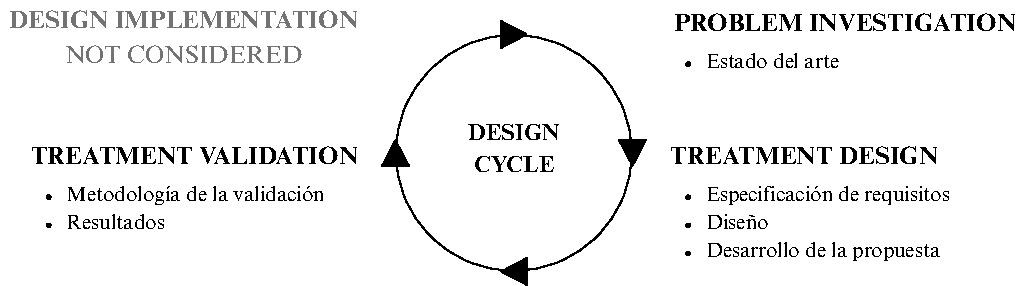
\includegraphics[width=0.9\textwidth]{tfgetsinf/images/Design cycle.pdf}
\caption{Ciclo de Diseño.}
\label{fig:ciclo_diseno}
\end{figure}

El ciclo de diseño se compone de tres fases principales: la investigación del problema, el diseño del tratamiento y la validación del tratamiento. Este conjunto de actividades se denomina ciclo de diseño porque los investigadores suelen iterar repetidamente sobre estas fases a lo largo de un proyecto de investigación basado en \textit{Design Science}.  A continuación, se explican las tres fases:
\begin{enumerate}
    \item Investigación del problema (\textit{Problem Investigation}): Se analiza en profundidad el contexto y los elementos clave del problema que se quiere abordar. En esta fase se identifican los \textit{stakeholders} y se definen los objetivos, así como los efectos y consecuencias que puede tener el desarrollo respecto a dichos objetivos. Además, se lleva a cabo un análisis del estado del arte, evaluando soluciones existentes y enfoques previos, lo que permite comprender mejor las limitaciones actuales y justificar la necesidad de una nueva propuesta.
    
    \item Diseño de la solución (\textit{Treatment Design}): En esta fase se genera la solución para dar respuesta a las limitaciones identificadas en la etapa anterior. Para ello, se lleva a cabo un proceso que abarca el diseño e implementación de la solución.
     
    \item Validación de la solución (\textit{Treatment Validation}): Se comprueba que la implementación del artefacto ha cumplido con los objetivos iniciales en la práctica. Algunas de las preguntas ligadas a esta fase se plantean el efecto real del tratamiento, la aceptación por parte de los usuarios y su eficacia. En definitiva, la validación permite detectar posibles limitaciones o áreas de mejora, lo que puede dar lugar a nuevas iteraciones sobre el diseño de la solución. 
\end{enumerate}

\subsection{Preguntas de investigación}
Para guiar el trabajo dentro de cada una de estas fases, se ha formulado una serie de preguntas de investigación. Estas preguntas están diseñadas para orientar el proceso de desarrollo, desglosar el problema y asegurar que la solución propuesta responde a las necesidades identificadas. 
Las preguntas han sido clasificadas en función de cada una de las fases metodológicas.

\textbf{Fase 1: Investigación del problema}
\begin{enumerate}
    \item ¿Cuál es la base de genética que sustentan los análisis PRS? 
    \item ¿Qué herramientas tecnológicas dan soporte a la ejecución de análisis PRS? 
    \item ¿Cuáles son las principales barreras y limitaciones que enfrentan los usuarios de estas herramientas tecnológicas? 
\end{enumerate}

\textbf{Fase 2: Diseño de la solución}
\begin{enumerate}
    \item ¿Qué requisitos debe cumplir una plataforma web para superar las barreras identificadas y facilitar el análisis PRS? 
    \item ¿Cuál es la arquitectura tecnológica más adecuada para esta plataforma? 
    \item ¿Cómo optimizar la carga, procesamiento y análisis de modelos PRS?     
\end{enumerate}

\textbf{Fase 3: Validación de la solución}
\begin{enumerate}
    \item ¿En qué medida la plataforma desarrollada cumple con los requisitos establecidos para superar las barreras identificadas en el análisis PRS?
    \item ¿Cuál es el nivel de usabilidad y utilidad percibida por los usuarios finales al interactuar con la plataforma?
\end{enumerate}

\subsection{\textit{Stakeholders}}
En este apartado se busca identificar los distintos grupos de interés del proyecto o \textit{stakeholders}. Según la metodología \textit{design science} (explicada en la sección~\ref{section:metodologia}), un \textit{stakeholder} es una persona, grupo de personas o institución que se ve afectada por el tratamiento de un problema. Identificarlos correctamente es fundamental, ya que de ellos surgen tanto los objetivos como las restricciones del proyecto que, a su vez, son la base para definir los requisitos que debe cumplir la solución desarrollada. 

Depende del tipo de problema, puede que los \textit{stakeholders} no sepan que lo son aún, por ejemplo, en los proyectos exploratorios, ya que los objetivos no están bien definidos al inicio de estos. En cambio, como en el caso de este proyecto, en los guiados por la utilidad, existen partes interesadas con objetivos definidos a los que la investigación debe contribuir. 

Se pueden encontrar diferentes tipos de \textit{stakeholders}; siendo identificados en este trabajo los siguientes para este proyecto: 
\begin{itemize}
    \item Investigadores en el ámbito de la genómica, más concretamente en análisis PRS. Serían los principales beneficiarios del desarrollo de esta plataforma, ya que son los que tienen unos objetivos claros acerca de la expectativa del resultado.
    \item Profesionales sanitarios como genetistas clínicos y asesores genéticos. A través de esta herramienta, podrían integrar los análisis PRS en su práctica clínica, gracias a que la plataforma ha sido diseñada para facilitar su uso por parte de profesionales sin conocimientos técnicos avanzados previos.
    \item Pacientes, quienes, aun sin interactuar directamente con la plataforma, se benefician de su uso por parte de profesionales clínicos, mejorando la prevención de enfermedades y diagnósticos. Su atención clínica en general se ve favorecida.
    \item Entidades colaboradoras, como centros de investigación, universidades, hospitales o biobancos, que podrían incorporar esta solución como parte de su infraestructura tecnológica.
\end{itemize}
De forma directa o indirecta, este grupo de personas o entidades se podría ver beneficiado por el desarrollo de la plataforma \textit{Phenoscore}.

\subsection{Aplicación de la metodología}
La aplicación de la metodología \textit{Design Science} se plasma en la organización del documento: cada fase metodológica encuentra su correspondencia en uno o varios capítulos, de modo que las cuestiones planteadas se van resolviendo de forma progresiva y coherente a lo largo de la memoria.

La primera fase, llamada investigación del problema, se ha resuelto en el Capítulo ~\ref{chap:investigación} (\nameref{chap:investigación}).

\begin{itemize}
    \item \textbf{Capítulo ~\ref{chap:introducción}. \nameref{chap:introducción}}: Se encarga de introducir y contextualizar el problema.También se presenta la motivación del proyecto, sus objetivos, la metodología empleada y los \textit{stakeholders} identificados.
    \item \textbf{Capítulo ~\ref{chap:investigación}. \nameref{chap:investigación}}: En este capítulo se da respuesta a las preguntas de investigación de dicha fase, analizando los fundamentos de los análisis PRS y se analizan los artefactos existentes que han dado algún tipo de solución a la ejecución de análisis PRS o a alguna fase de su configuración y se comparan esas soluciones con la propuesta presentada.
\end{itemize}

La segunda fase, llamada diseño de la solución, se ha resuelto en el capítulo ~\ref{chap:diseño} (\nameref{chap:diseño}).

\begin{itemize}
    \item \textbf{Capítulo ~\ref{chap:diseño}. \nameref{chap:diseño}}: en la sección ~\ref{section:especificación} se han detectado las oportunidades de mejora y se han definido las características y funcionalidades necesarias para el desarrollo a través de los requisitos como: historias de usuario, requisitos funcionales y no funcionales. Posteriormente, se ha realizado el modelado conceptual junto con las posibles soluciones identificadas y la solución propuesta.
    
    Por lo que se refiere a la tecnología y el diseño de la interfaz, ambas cuestiones se han resuelto en la sección ~\ref{section:diseño}; se han descrito las herramientas que se van a usar junto con la estructura de la solución. Además, a través de los \textit{mockups} se ha representado la idea del diseño visual de la aplicación.

    Por otro lado, en la sección ~\ref{section:desarrollo} se ha llevado a cabo la implementación de las funcionalidades anteriormente identificadas en el análisis.
    
\end{itemize}

La última fase, llamada validación de la solución, se ha resuelto en el capítulo ~\ref{chap:pruebas} (\nameref{chap:pruebas}).

\begin{itemize}
    \item \textbf{Capítulo ~\ref{chap:pruebas}. \nameref{chap:pruebas}}: se detalla la metodología de validación, los participantes, el procedimiento seguido y los instrumentos de medición empleados. Se presentan los resultados, incluyendo la validación funcional, la evaluación de requisitos no funcionales, la aceptación tecnológica y la matriz de trazabilidad. Además, se analiza si la solución ha resultado satisfactoria respecto a las expectativas y necesidades de los \textit{stakeholders}.
\end{itemize}

Por último, se han presentado las conclusiones del trabajo en el capítulo ~\ref{chap:conclusiones} 
(\nameref{chap:conclusiones}).

\begin{itemize}
    \item \textbf{Capítulo ~\ref{chap:conclusiones}. \nameref{chap:conclusiones}}: se sintetizan los resultados del trabajo, se establecen relaciones con las competencias del grado y se señalan posibles mejoras y líneas de evolución futura.
\end{itemize}